% \documentclass[aip,jcp,preprint,unsortedaddress,a4paper,onecolum]{revtex4-1}
\documentclass[aip,jcp,a4paper,reprint,onecolumn]{revtex4-1}
% \documentclass[aps,pre,twocolumn]{revtex4-1}
% \documentclass[aps,jcp,groupedaddress,twocolumn,unsortedaddress]{revtex4}

\usepackage[fleqn]{amsmath}
\usepackage{amssymb}
\usepackage[dvips]{graphicx}
\usepackage{color}
\usepackage{tabularx}
\usepackage{algorithm}
\usepackage{algorithmic}

\makeatletter
\makeatother

\newcommand{\recheck}[1]{{\color{red} #1}}
\newcommand{\redc}[1]{{\color{red} #1}}
\newcommand{\bluec}[1]{{\color{blue} #1}}
\newcommand{\vect}[1]{\textbf{\textit{#1}}}
\newcommand{\dd}[1]{\textsf{#1}}

\newcommand{\AT}{{\textrm{{AT}}}}
\newcommand{\EX}{{\textrm{EX}}}
\newcommand{\CG}{{\textrm{CG}}}
\newcommand{\HY}{{\Delta}}
\newcommand{\rdf}{{\textrm{rdf}}}
\newcommand{\corr}{C^{(3)}}



\begin{document}

\title{The reliability of AdResS in performing  Molecular Dynamics in a Grand Canonical fashion}
\author{Han Wang}
\affiliation{Institute for Mathematics, Freie Universit\"at Berlin, Germany}
\author{Carsten Hartmann}
\affiliation{Institute for Mathematics, Freie Universit\"at Berlin, Germany}
\author{Christof Sch\"utte}
\affiliation{Institute for Mathematics, Freie Universit\"at Berlin, Germany}
\author{Luigi Delle Site}
\email{luigi.dellesite@fu-berlin.de}
\affiliation{Institute for Mathematics, Freie Universit\"at Berlin, Germany}

\begin{abstract}
\end{abstract}

\maketitle

\newpage
\section{The third order correlation function}

The three-body correlation function of a molecular system is defined by:
\begin{align}
  \corr (\vect s_1, \vect s_2, \vect s_3)
  =
  \frac1{\rho(\vect s_1)\rho(\vect s_2)\rho(\vect s_3)}
  \big\langle
  (\hat\rho(\vect s_1) - \rho(\vect s_1))\cdot
  (\hat\rho(\vect s_2) - \rho(\vect s_2))\cdot
  (\hat\rho(\vect s_3) - \rho(\vect s_3))
  \big\rangle
\end{align}
where the transient density distribution $\hat\rho(\vect s)$ and the
average density distribution $\rho(\vect s)$ are given
by:
\begin{align}
  \hat\rho(\vect s) = \sum_{i=1}^N\delta(\vect s - \vect r_i)
  \quad\textrm{and}\quad
  \rho(\vect s) = \big\langle \hat\rho(\vect s)\big\rangle.
\end{align}
By assuming that the system is homogeneous, 
after some straightforward algibra, one can show that
\begin{align}
  \corr (\vect s_1, \vect s_2, \vect s_3)
  =
  \frac1{\rho^3}\,\rho(\vect s_1, \vect s_2, \vect s_3) -
  \frac1{\rho^2}\,\big[
  \rho(\vect s_1, \vect s_2) +
  \rho(\vect s_1, \vect s_3) +
  \rho(\vect s_2, \vect s_3)
  \big] + 2
\end{align}
where
\begin{align}
  \rho(\vect s_1, \vect s_2)
  =
  \big\langle
  \hat\rho(\vect s_1)\,  \hat\rho(\vect s_2)
  \big\rangle
  \quad\textrm{and}\quad
  \rho(\vect s_1, \vect s_2, \vect s_3)
  =
  \big\langle
  \hat\rho(\vect s_1)\,  \hat\rho(\vect s_2)\, \hat\rho(\vect s_3)
  \big\rangle  
\end{align}
Since $g (\vect s_1, \vect s_2) = \rho(\vect s_1, \vect s_2)/\rho^2$
is the two-body radial distribution function, 
\begin{align}
  \corr (\vect s_1, \vect s_2, \vect s_3)
  =
  \frac1{\rho^3}\,\rho(\vect s_1, \vect s_2, \vect s_3) -
  \big[
  g(s_{12}) +
  g(s_{13}) +
  g(s_{23})
  \big] + 2
\end{align}
where for example $s_{12} = \vert \vect s_1 -\vect s_2\vert$.

Since we assume the system is homogeneous, visulization of this high-dimensional
distribution is simplified: We first fix the distance between molecule 1 and 2 (Mol
1 and 2 in Fig.~\ref{fig:tmp3}), then plot the correlation function with
respect to the position of the third molecule (Mol 3 in
Fig.~\ref{fig:tmp3}).  The position of Mol 3 can be described by
the variables $h_1$ and $h_2$ in Fig.~\ref{fig:tmp3}, which are
the projection of Mol~3's position on the to the
axis defined by Mol 1 and 2, see Fig.~\ref{fig:tmp3}.

\begin{figure}
  \centering
  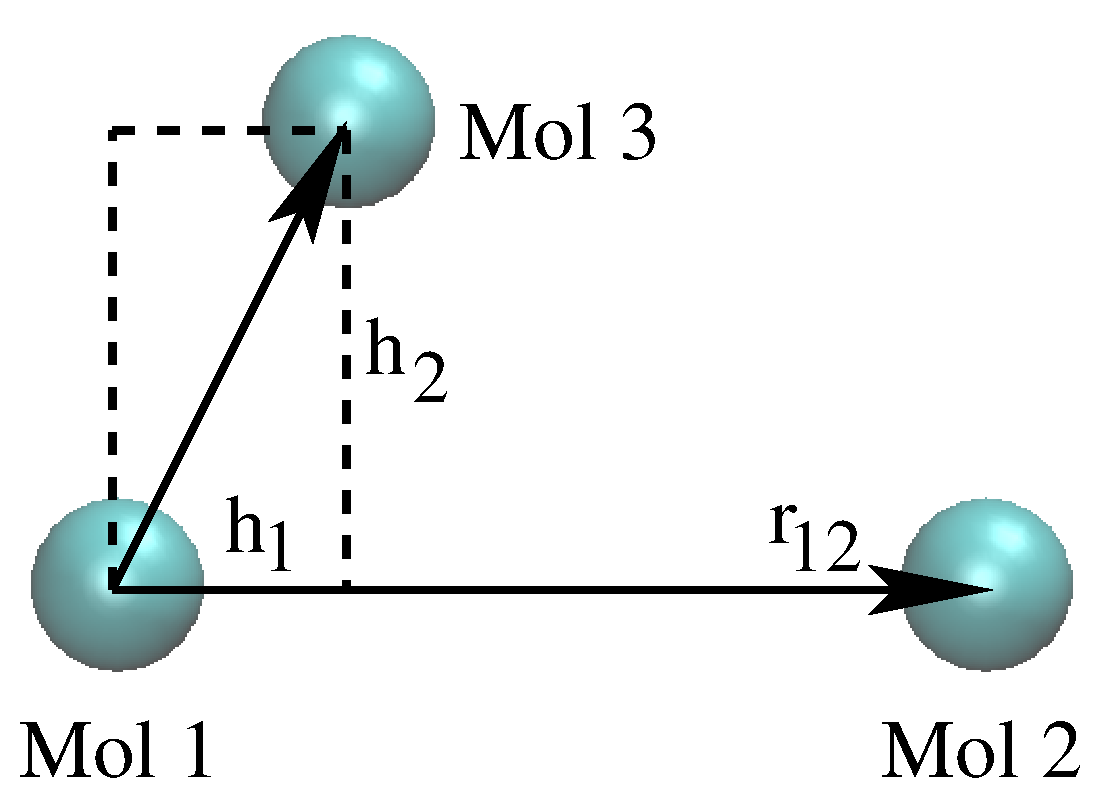
\includegraphics[width=0.3\textwidth]{3mol.eps}
  \caption{The schematic plot of the 3-body RDF.}\label{fig:tmp3}
\end{figure}

For numerical result, please see Fig.~\ref{fig:tmp1} and \ref{fig:tmp2}.
\begin{figure}
  \centering
  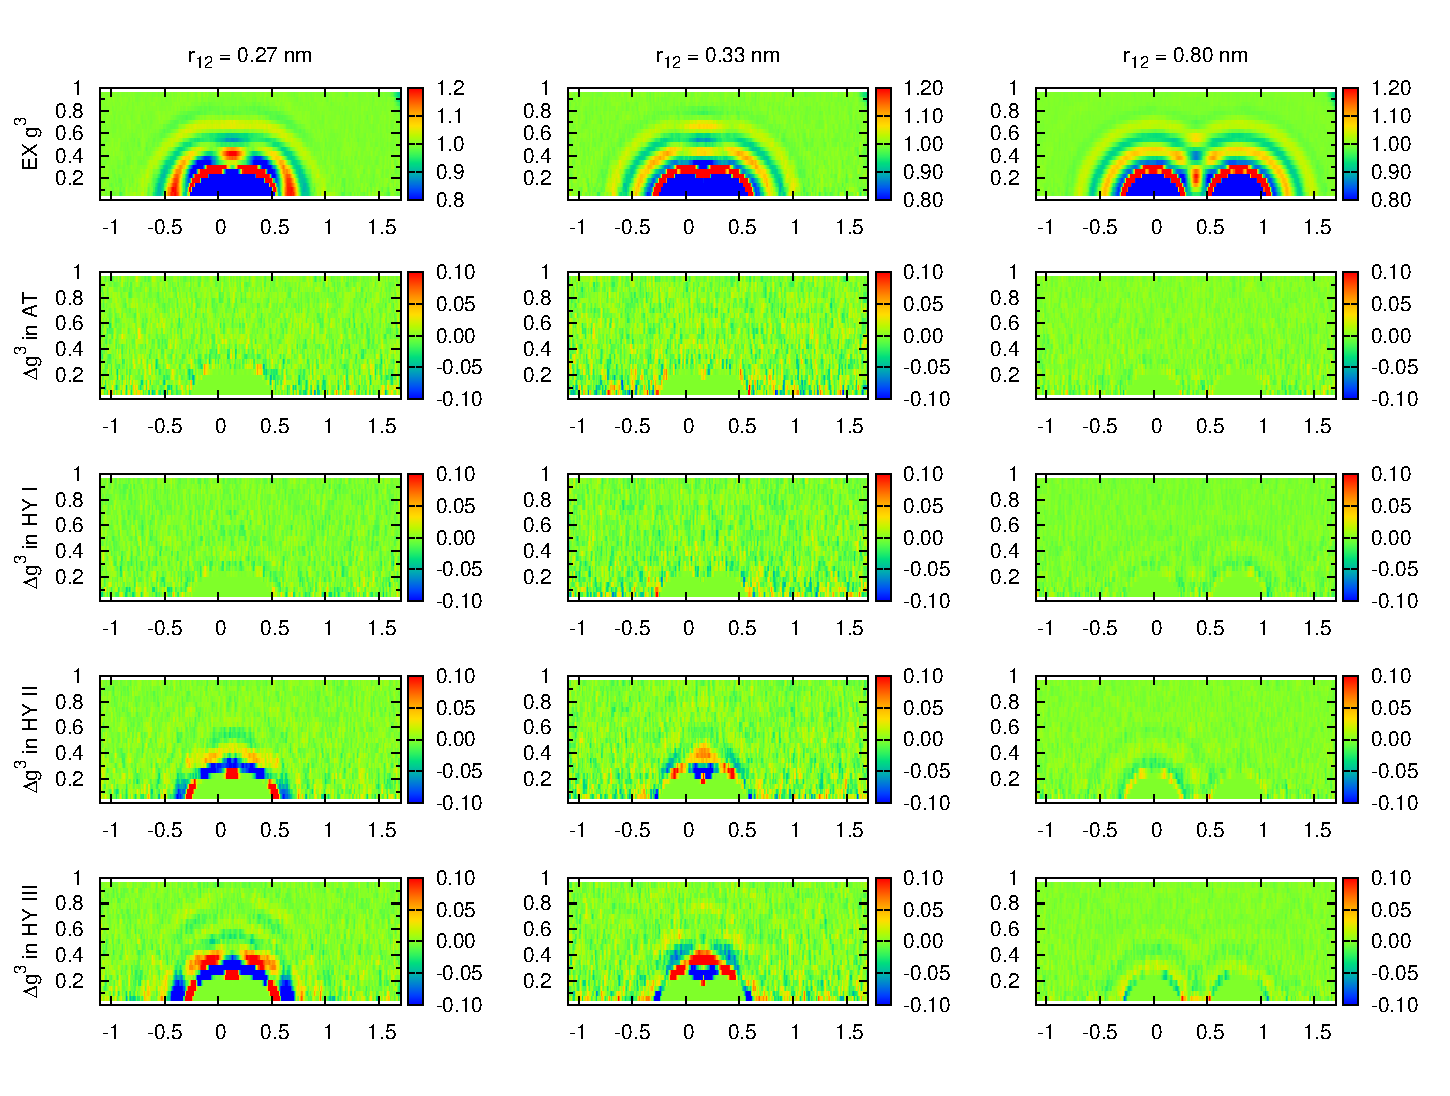
\includegraphics[width=0.9\textwidth]{fig-rdf3-diff.eps}
  % 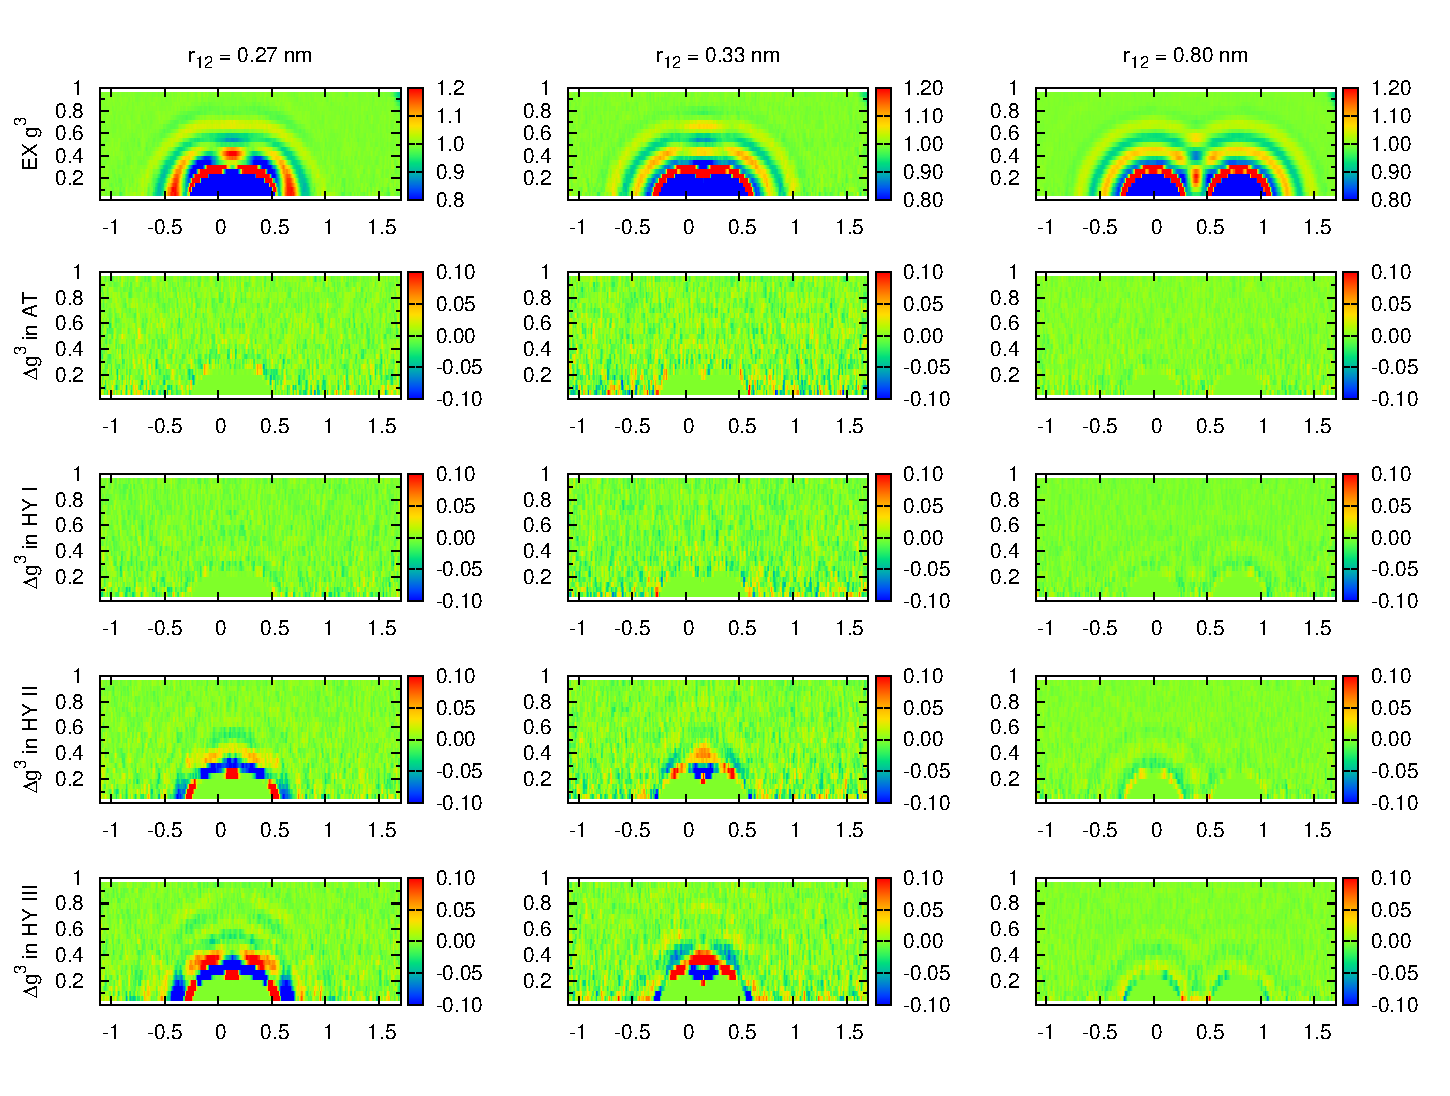
\includegraphics[]{fig-rdf3-diff.eps}
  \caption{The 3-body correlation function.  The 1st row corresponds to the reference all atom simulation.
    From the 2nd to 5th row:
    The difference between the function calculated in AdResS in the AT, HY I, HY II, and HY III
    regions, respectively, and the reference function of the full atomistic case.
    Different columns give different distances between
    the first two molecules: from left to right $r_{12} =
    0.27\,\textsf{nm},\ 0.33\,\textsf{nm},\  
    0.80\,\textsf{nm}$.  The $x$ axis corresponds to the variable $h_1$, while $y$
    axis is the variable $h_2$ (see the Appendix~\ref{app:3} for the
    definition of these variables).  The magnitude of the function is indicated by
    different colors. Essentially for the atomistic region of AdResS the difference is negligible.
  }
  \label{fig:tmp1}
\end{figure}
\begin{figure}
  \centering
  \includegraphics[width=0.9\textwidth]{fig-wca-rdf3-diff-ex-hy1.eps}
  \caption{The 3-body correlation of WCA AdResS in the AT
    and HY I regions.
    The difference with respect to the full atomistic reference
    (see the fist line of Fig.~\ref{fig:tmp1})
    is plotted in this figure. From left to right, the distance
    between the first two molecules are $r_{12} =
    0.27\,\textsf{nm},\ 0.33\,\textsf{nm},\  
    0.80\,\textsf{nm}$, respectively.
  }
  \label{fig:tmp2}
\end{figure}


\section{About the efficiency of the }

We use the standard test particle insertion method to calculate the
chemical potential of the atomistic water model, see the lower panel
of Fig.~\ref{fig:tmp4}. We used the equilibirum trajectory of length
8~\textsf{ns}. The coordinates of water molecules were recorded every
0.2~\textsf{ps}.  In each frame, $10^5$ test particles were inserted
at random position of the system. For each insertion, $10^5$ radomly
chosen orientations were tried. The convergence of the result were very
slow, even at 8~\textsf{ns} the it is not satisfactorily converged.
Comparing with test particles insertion, the AdResS leads a very
efficient insertion of particles: in each 1~\textsf{ps} time interval,
on average 34 water molecules were inserted into the atomistic region. Some of
them were immediately send back, because of a unfavorable entering
configuration.  To investigate the proper insertion, we consider the
time interval of 1~\textsf{ns}, and find 832 out of 3456 molecules
were firstly in either the HY or CG region, and then travelled to the
AT region and stayed there for longer than 60~\textsf{ps}, which
indicates a mean square root displacement of roughly 1~\textsf{nm}
in the AT region.


\begin{figure}
  \centering
  \includegraphics[]{fig-tpi.eps}
  \caption{The chemical potential calculated by the test particle insertion method}
  \label{fig:tmp4}
\end{figure}


\begin{table}
  \centering
  \begin{tabular}{l|l|l|l|l}
    & Sys. size ($\textsf{nm}^3$)
    & Traj. length (\textsf{ns})
    & CPU perf. (G FLOPS)
    & CPU time (hours)\\    \hline
    AdResS   &$29.9\times3.7\times3.7$ & 1 &  4.1 & 3.1\\
    EX water & $3.7\times3.7\times3.7$ & 8 & 24.7 & 4.5 (traj.) + 36.7 (TPI)\\
    CG water & $3.7\times3.7\times3.7$ & 8 &  5.8 & 1.0 (traj.) + 3.4 (TPI)\\
  \end{tabular}
  \caption{CPU time.
    The AdResS simulation contains 13824 molecules, while both EX and CG
    water simulations contain 1728 molecules. In the AdResS simulation,
    the size of the AT + HY regions is roughly the same as the EX water
    simulation box.
    ``Sys. size'' means the size of the box used in the simulaiton.
    ``Traj. length'' means the equilibirum trajectory
    used for the test particle insertion. Along the trajectories, frames
    of configurations were recoreded every 0.2~\textsf{ps}.
    ``CPU perf.'' is the CPU performance
    counted by the floating-point operations per second (FLOPS).
    ``CPU time'' the is wall clock time spend on the simulation.
    For the particle insertion simulation, the CPU time is counted by two
    parts: the time of generating the equilibirum trajectories (traj.)
    and the time of test particle insertion (TPI).
  }
  \label{tab:tmp1}
\end{table}
%    WCA      & $3.7\times3.7\times3.7$ & 8 & 0.2 (traj.) + 0.5 (TPI)\\

\section*{References}
\bibliography{ref}{}
\bibliographystyle{unsrt}





\end{document}